Once the theoretical update equations are implemented, a validation procedure is needed to confirm the legitimacy of the simulations. The code is validated with a test including a lossy region at the right side of the grid, while the left side is loss-less. In this case, the layer is composed of cerebral tissue (relative permittivity $\varepsilon_r$, conductivity $\sigma$) and the source of excitation is an harmonic source at frequency $f$ (this validation will be a first step to introduce the SAR simulation). The values of the parameters are summarised in \autoref{tab:valpar}. The simulation will be considered valid if the wavelength and the attenuation in the lossy layer match the expected theoretical results.

%The validation criteria will be on the verification of the wavelength value and the loss characteristic in the layer.

\begin{table}[H]
    \centering
    $\begin{array}{|c|c|}
    \hline
    \varepsilon_r & 43 \\\hline
    \sigma & \SI{1.3}{\siemens\per\meter}\\\hline
    f & \SI{915}{\mega\hertz}\\\hline
    \end{array}$
    \caption{Validation parameters}
    \label{tab:valpar}
\end{table}

The wavelength in the lossy layer is defined as
\begin{equation}
\label{eq:valid:lambdal}
    \lambda_l = \frac{v_\varphi}{f}\quad\text{where}\quad\begin{cases*}
    v_\varphi & propagation/phase velocity \\
    f & wavelength frequency
    \end{cases*}
\end{equation}
Knowing that 
\begin{equation}\label{eq:valid:vandB}
v_\varphi=\frac{\omega}{\beta}\quad\text{and}\quad \beta=\omega\sqrt{\frac{\mu_0\varepsilon_r\varepsilon_0}{2}\left[\sqrt{1+\left(\frac{\sigma}{\omega\varepsilon_r\varepsilon_0}\right)^2}+1\right]}
\end{equation}
by coupling \eqref{eq:valid:lambdal} and \eqref{eq:valid:vandB}, one finds $\lambda_l\approx\SI{48}{\milli\meter}$. Being the wavelength of interest, $\Delta x=\frac{\lambda_l}{10}=\SI{4.8}{\milli\meter}$ and $\Delta t=S_c\frac{\Delta x}{c}\approx\SI{11.32}{\nano\second}$.  

The loss can be characterised by the skin depth $\delta = \frac{1}{\alpha}$, where

\begin{equation}
\alpha = \omega\sqrt{\frac{\mu_0\varepsilon_r\varepsilon_0}{2}\left[\sqrt{1+\left(\frac{\sigma}{\omega\varepsilon_r\varepsilon_0}\right)^2}-1\right]}
\end{equation}

$\alpha$ representing the rate of decay of the wave amplitude (represented \autoref{fig:valid:alphaeg}). In that way, $\alpha\approx\SI{35.91}{\per\meter}$ and $\delta\approx\SI{2.79}{\centi\meter}$.

\begin{figure}[H]
\centering
    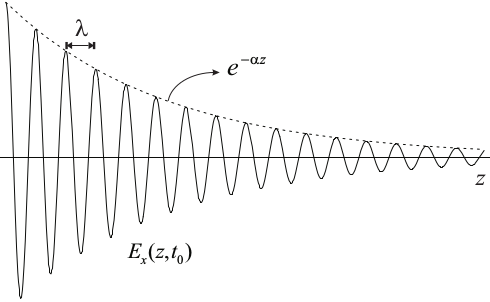
\includegraphics[width=.7\textwidth]{img/alpha}
     \caption{Decay of the wave amplitude in a lossy layer}
     \label{fig:valid:alphaeg}
\end{figure}

The different parameters needed to run the simulation are then defined, such as the number of point per wavelength $N_\lambda$ (source excitation) and the loss parameter used in the code of \autoref{sec:codefields} (equals to $\frac{\sigma\Delta t}{2\varepsilon}$ since the magnetic effects are neglected ($\sigma_m=0$, $\mu_r= 1$)).

\begin{equation}
N_\lambda=\frac{\lambda}{\Delta x} = \frac{c}{f\Delta x} \approx \num{68.20}
\end{equation}
\begin{equation}
\text{LOSS} = \frac{\pi}{N_\lambda}S_c\sqrt{\left(1+\frac{N_\lambda^2}{2\pi^2N_L^2\varepsilon_r\mu_r}\right)^2 +1} \approx\num{19.35e-3}
\end{equation} 
where
\begin{equation}
N_L = \frac{\delta}{\Delta x}
\end{equation}

The result of the simulation is shown in \autoref{fig:valid:SAR_Layer}. The electric field after the lossy layer on a horizontal line $E_z(x,100,t')$ is shown in  \autoref{fig:valid:SAR_Layer_x}. On \autoref{fig:valid:SAR_Layer_x}, the \emph{Curve Fitting} MATLAB tool was used to fit the exponential decay. $\lambda_l$ and $\alpha$ can be deduced: $\lambda_l\approx\SI{48}{\milli\meter}$ and $\alpha\approx \SI{35.26}{\per\meter}$, as expected (neglecting graphical fitting errors).

\begin{figure}[H]
\centering
    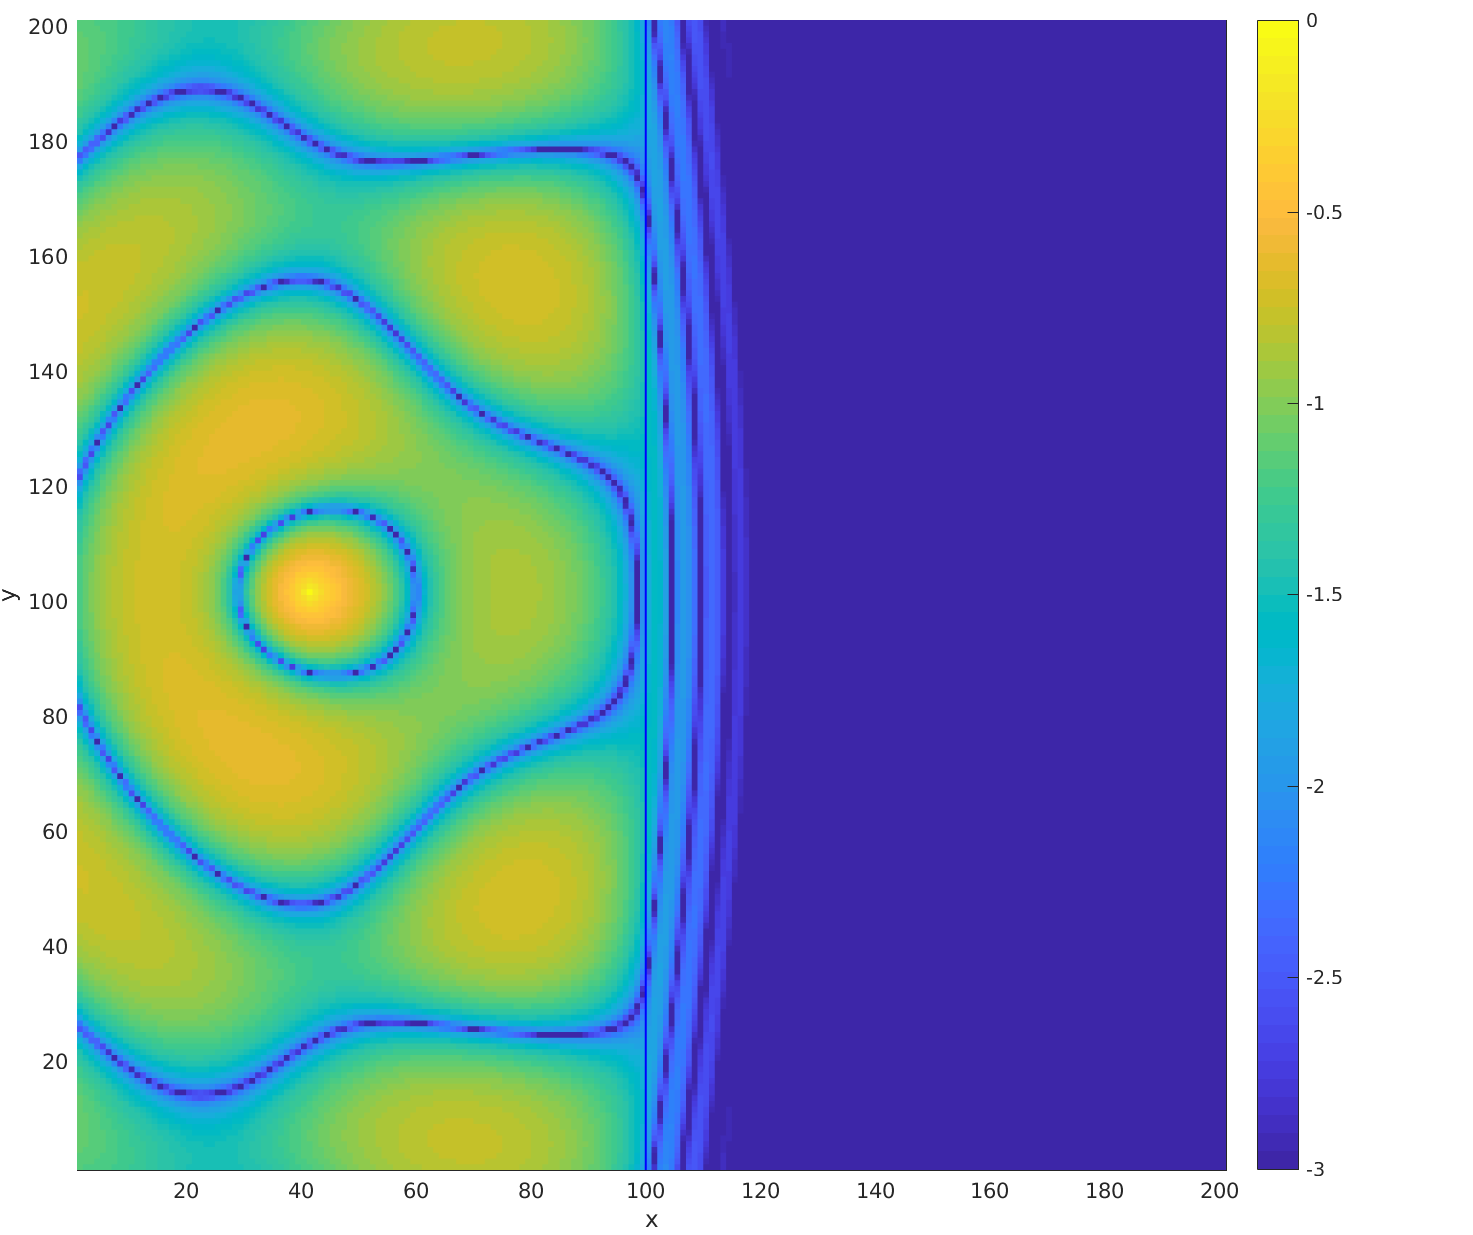
\includegraphics[width=.8\textwidth]{img/SAR_layer_im.pdf}
     \caption{Decay of the wave amplitude in a lossy layer of cerebral tissue}
     \label{fig:valid:SAR_Layer}
\end{figure}
\begin{figure}[H]
\centering
    \includegraphics{img/SAR_Layer.tex}
     \caption{Wave propagation with a lossy layer of cerebral tissue}
     \label{fig:valid:SAR_Layer_x}
\end{figure}

Hence, the simulation is validated and more advanced simulations can be designed.